\subsection{Gradient Dynamics with Feature Learning}
\begin{align}
&\text{Parameter}&\dot{\Theta}_t&=&-\sum_{s=1}^n \psi_{x,t}e_t(s)\\
&\text{NPF}              &\dot{\phi}_{x_s,t}(p)&=&x(\I_0(p))\sum_{\theta\in\Theta}\partial_{\theta}A_t(x_s,p)\dot{\theta}_t,\forall p\in[P], s\in[n]\\
&\text{NPV}              &\dot{v}_t(p)&=&\sum_{\theta\in\Theta}\partial_{\theta}v_t(p)\dot{\theta}_t,\forall p\in[P]\\
&\text{Kernel}              &K_{\Theta}=(K^v_{\Theta}+K^{\phi}_{\Theta}+(\Psi^v_{\Theta})^\top \Psi^{\phi}_{\Theta}+(\Psi^v_{\Theta})^\top\Psi^{\phi}_{\Theta})\\
&\text{Error}     &\dot{e}_t&=&-(K^v_t+K^{\phi}_t+(\Psi^v_{t})^\top \Psi^{\phi}_{t}+(\Psi^v_{t})^\top\Psi^{\phi}_{t})e_t
\end{align}
\subsection{Relation between $K^v_{\Theta}$, $K^{\phi}_{\Theta}$ and $K^{(d)}$ }
\subsection{Role of gates in feature learning}
$4.$ The soft-ReLU activation plays a key part: note that, in prior works, in the expression for the limit NTK $K^{(d)}$ in \eqref{eq:ntkold}, $\dot{\chi}$ is either a Heaviside step function or a logit function. Both these functions capture the \emph{on/off} behaviour of the gates, and hence the $K^{(d)}$ captures only the flow of value gradient through the active sub-networks. On the contrary, in the case of soft-ReLU (see row $3$ of \Cref{tb:compare}), $\dot{\chi}_{SR}$ contains both the \emph{on/off} information via the $\dot{\chi}_{SP}$ term as well as the information on the dynamics of sensitive gates via the $\dot{G}_{SR}$ term.
\FloatBarrier
\begin{figure*}[h]\centering
%\begin{minipage}{0.78\columnwidth}
\resizebox{\columnwidth}{!}{
\begin{tabular}{ccc}
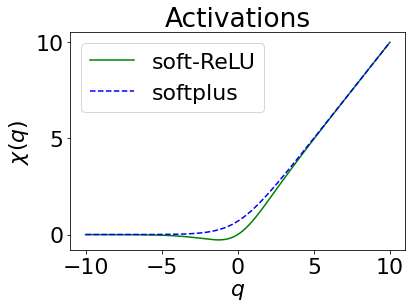
\includegraphics[scale=0.4]{figs/act.png}
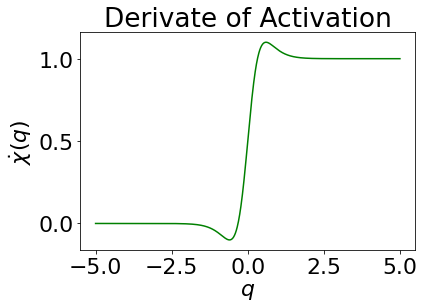
\includegraphics[scale=0.4]{figs/der-act.png}
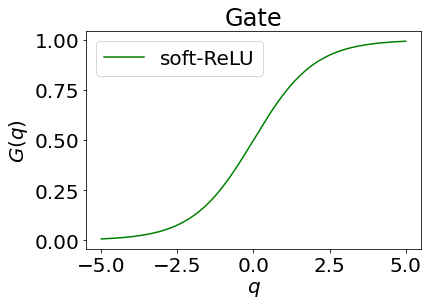
\includegraphics[scale=0.4]{figs/gate.png}
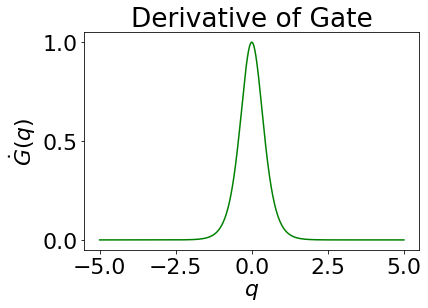
\includegraphics[scale=0.4]{figs/der-gate.png}
%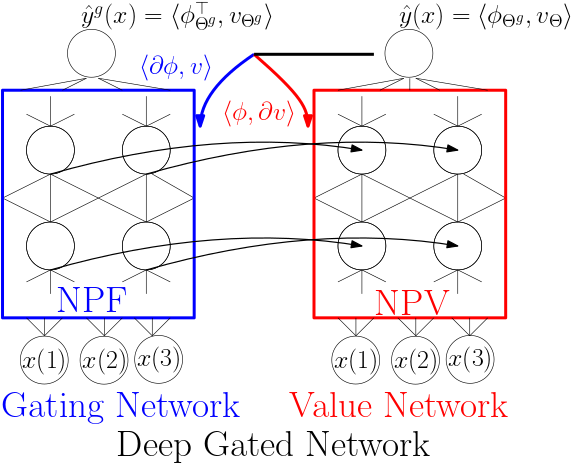
\includegraphics[scale=0.5]{figs/nntwin-blck.png}
%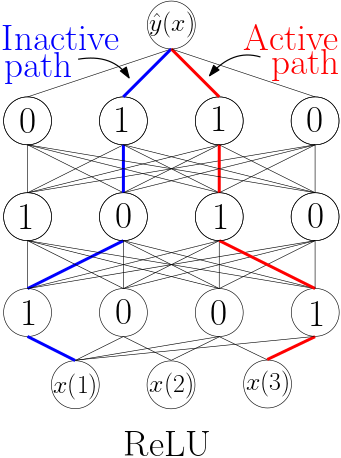
\includegraphics[scale=0.5]{figs/nn.png}
%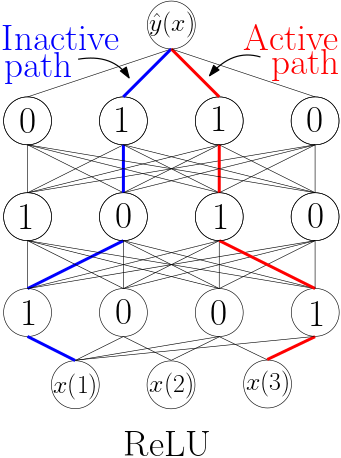
\includegraphics[scale=0.5]{figs/nn.png}
\end{tabular}
}
%\end{minipage}
%\begin{minipage}{0.18\columnwidth}
%\resizebox{\columnwidth}{!}{
%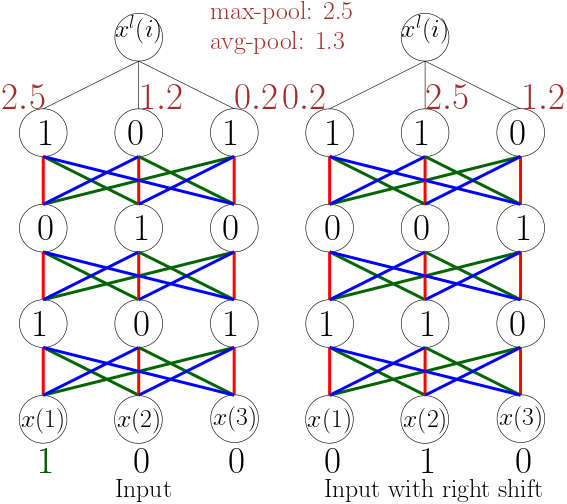
\includegraphics[scale=0.5]{figs/nnconv.png}
%}
%\end{minipage}
\caption{Activations and Gates}
\label{fig:actgate}
\end{figure*}
$5.$ Plugging the soft-ReLU instead of softplus/ReLU in \eqref{eq:ntkold} will indeed bring in the additional terms related to gate dynamics (see last row of \Cref{tb:compare}) in $K^{(d)}$. However, note that $K^{(d)}$ is a single matrix, and only due to the `path-view', we can identify its components namely $K^v_{\Theta}$, and $K^{\phi}_{\Theta}$ which have completely different functions.
